\documentclass{article}
\usepackage[left=3cm,right=3cm,top=2cm,bottom=2cm]{geometry}
\usepackage{makeidx}         % allows index generation
\usepackage[pdftex]{graphicx,color}          % standard LaTeX graphics tool
\DeclareGraphicsRule{.pdftex}{pdf}{.pdftex}{}
                             % when including figure files
\usepackage{multicol}        % used for the two-column index
\usepackage[bottom]{footmisc}% places footnotes at page bottom

\usepackage{booktabs}
\usepackage{arydshln}
\setlength\dashlinedash{0.5pt}
\setlength\dashlinegap{1.5pt}
\setlength\arrayrulewidth{0.3pt}

\usepackage{amssymb}
\usepackage{amsmath}
\usepackage{pifont}
\usepackage{bm}
\usepackage{cancel}
\usepackage{multirow}
\usepackage{amsmath}
\usepackage{epstopdf}
\usepackage{float}
\usepackage{subfigure}
\usepackage[caption=false,font=footnotesize]{subfig}

\usepackage{listings}


\DeclareMathOperator*{\argmin}{arg\,min}

\DeclareGraphicsExtensions{.eps, .pdf, .png, .jpg}
\graphicspath{{./images/Ex1/}, {./images/Ex2/}, {./images/Ex3/}, {./images/Ex4/}, {./images/Ex5/}, {./images/Ex6/},{./}}

\newcommand{\red}[1]{{\color{red}#1}}
\renewcommand{\vec}[1]{\bm{#1}}
\newcommand{\mat}[1]{\bm{#1}}
\newcommand{\cframe}[1]{$\langle #1 \rangle$}
\newcommand{\prescript}[2]{\phantom{}^{#1}_{#2}}

\newcommand\frontmatter{%
    \cleardoublepage
%%  \@mainmatterfalse
  \pagenumbering{roman}}
\newcommand\mainmatter{%
    \cleardoublepage
%%  \@mainmattertrue
  \pagenumbering{arabic}}
%%%%%%%%%%%%%%%%%%%%%%%%%%%%%%%%%%%%%%%%%%%%%%%%%%%%%%%%%%%%%%%%%%%%%

\begin{document}
\frontmatter
\onecolumn
\vskip 1cm
%\pagestyle{empty}
\begin{center}
\huge \textsc{Cooperative Robotics}\\
\vskip 1cm

\skip 0.5cm

\vskip 5cm

\normalsize
Authors: Piccinini Davide, Porta Francesco and Gotelli Andrea \\
EMAILs: 4404040@studenti.unige.it, 4376330@studenti.unige.it, 4343879@studenti.unige.it \\
Date: 21/12/2020
\end{center}
\clearpage
\mainmatter
\section*{General notes}

\begin{itemize}
	\item Exercises 1-4 are done with the ROBUST matlab main and unity visualization tools. Exercises 5-6 are done with the DexROV matlab main and unity visualization tools.
	\item Comment and discuss the simulations, in a concise scientific manner. Further comments, other than the questions, can be added, although there is no need to write 10 pages for each exercise.
	\item Aid the discussion with screenshots of the simulated environment (compress them to maintain a small overall file size), and graphs of the relevant variables (i.e. activation functions of inequality tasks, task variables, and so on). Graphs should always report the units of measure in both axes, and legends whenever relevant.
	\item Report the thresholds whenever relevant.
	\item Report the mathematical formula employed to derive the task jacobians and the control laws when asked, including where they are projected.
	\item If needed, part of the code can be inserted as a discussion reference.
\end{itemize}


Use the following template when you need to discuss the hierarchy of tasks of a given action or set of actions:
\begin{table}[htb]
	\caption{Example of actions/hierarchy table: a number in a given cell represents the priority of the control task (row) in the hierarchy of the control action (column). The type column indicates whether the objective is an equality (E) or inequality (I) one.}
	\label{tbl:actions_table}
	\begin{center}
		\footnotesize
		\begin{tabular}{ccccc}
			\toprule
			Task & Type & $\mathcal{A}_{1}$ & $\mathcal{A}_{2}$ & $\mathcal{A}_{3} $	 \\
			\midrule
			Task A                    & I & 1 &   & 1  \\
			\hdashline
			Task B                & I & 2 & 1 &   \\
			\hdashline
			Task C                       & E &   & 2 & 2   \\

			\bottomrule
		\end{tabular}
	\end{center}
\end{table}% %

\clearpage


\section{Exercise 1: Implement a “Safe Waypoint Navigation” Action.}

\subsection{Adding a vehicle position and attitude control objective}
Initialize the vehicle far away from the seafloor. An example position could be
\begin{displaymath}
\begin{bmatrix} 10.5 & 35.5 & -36 & 0 & 0 & \pi/2\end{bmatrix}^\top
\end{displaymath} 
Give a target position that is also sufficiently away from the seafloor, e.g.,
\begin{displaymath}
\begin{bmatrix} 10.5 & 37.5 & -38 & 0 & 0 & 0 \end{bmatrix}^\top
\end{displaymath}

Goal: Implement a vehicle position and attitude control task, and test that the vehicle reaches the required position and orientation.


\subsubsection{Q1: What is the Jacobian relationship for the Vehicle Position and Attitude control task? How was the task reference computed?}

The Vehicle Position and Attitude control task controls both the position and the attitude of the vehicle in order to make them converge to a desired goal position. Since there are in principle one goal for the position and another for the attitude, there are two Jacobian matrices, one for each control problem. \\
Since the goal position and goal attitude are expressed with respect to the world frame, our task reference vector $ \dot{x} = J\dot{y} $ needs to be projected on the world frame too. \\
For this reason, since the control vector $ \dot{y} = \begin{bmatrix} \dot{q} & \dot{v} & \dot{\omega}\end{bmatrix}^\top $ is projected in the vehicle frame, the two Jacobian matrices will be:
\begin{gather*}
uvms.Jv\_pos = \begin{bmatrix} zeros(3, 7) & uvms.wTv(1:3, 1:3) & zeros(3,3)\end{bmatrix}^\top \\
uvms.Jv\_att = \begin{bmatrix} zeros(3, 7) & zeros(3, 3) & uvms.wTv(1:3, 1:3)\end{bmatrix}^\top
\end{gather*}

The task reference vector must be in the form $ \dot{\bar{x}} = \lambda(\bar{x} - x), \lambda > 0 $, where the reference value $ \bar{x} $ represents the desired value and $ x $ is the current value. In our case the desired value is the goal position (or attitude) obtained with the \textit{CartError()} function and the current value is the current position (or attitude). \\
The two task reference vectors are computed in this way:
\begin{gather*}
[ang, lin] = CartError(uvms.wTg\_v , uvms.wTv);\\
uvms.xdot.v\_pos = Saturate(0.5 * lin, 0.5);\\
uvms.xdot.v\_att = Saturate(0.5 * ang, 0.5);
\end{gather*}
Where $ uvms.wTg\_v $ and $ uvms.wTv $ are respectively the transformation matrix of the goal frame with respect to the world frame and the transformation matrix of the vehicle frame with respect to the world frame. 

\subsubsection{Q2: What is the behaviour if the Horizontal Attitude is enabled or not? Try changing the initial or target orientation in terms of roll and pitch angles. Discuss the behaviour.}
In order to observe the robot behaviour we considered three cases:
\begin{itemize}
	\item Case 1: Horizontal attitude disabled and original initial and target configurations as stated in the exercise description;
	\item Case 2: Horizontal attitude enabled, original initial configuration but different target one, which is the following 
	\begin{gather*}
		\begin{bmatrix} 10.5 & 37.5 & -38 & \pi/3 & \pi/3 & 0\end{bmatrix}^\top
	\end{gather*}
	\item Case 3: Horizontal attitude enabled and different initial and target configurations, which are the following 
	\begin{gather*}
		\begin{bmatrix} 10.5 & 35.5 & -36 & \pi/3 & \pi/3 & \pi/2\end{bmatrix}^\top \\
		\begin{bmatrix} 10.5 & 37.5 & -38 & \pi/3 & \pi/3 & 0\end{bmatrix}^\top
	\end{gather*}
\end{itemize}

{\large \textbf{Case 1}} \\
In this case the behavior is normal, the robot reaches the target position and attitude without problems.

\begin{figure}[H]
	\centering
	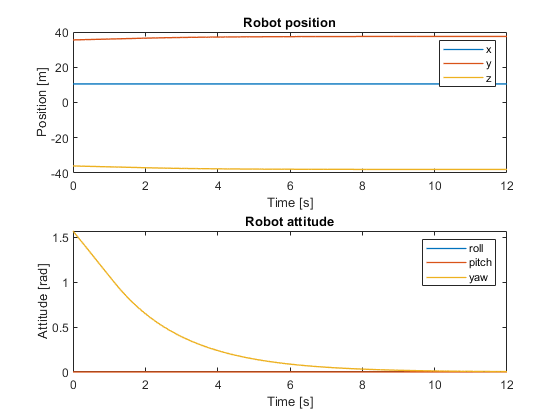
\includegraphics[width=0.7\linewidth]{images/Ex1/HorAtt_Disabled_SameStartpos_SameEndpos_PosAndAtt}
	\caption{The robot moves in the Y and Z directions and the yaw angle converges to zero.}
	\label{fig:q2case1a}
\end{figure}
\begin{figure}[H]
	\centering
	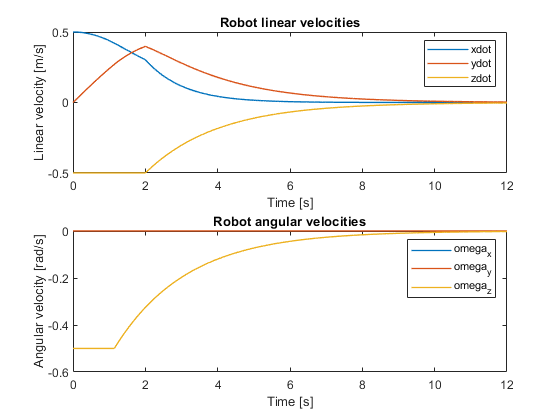
\includegraphics[width=0.7\linewidth]{images/Ex1/HorAtt_Disabled_SameStartpos_SameEndpos_LinAngVelocities}
	\caption{After an initial transient phase, all the velocities converge to zero.}
	\label{fig:q2case1b}
\end{figure}

\begin{figure}[H]
	\centering
	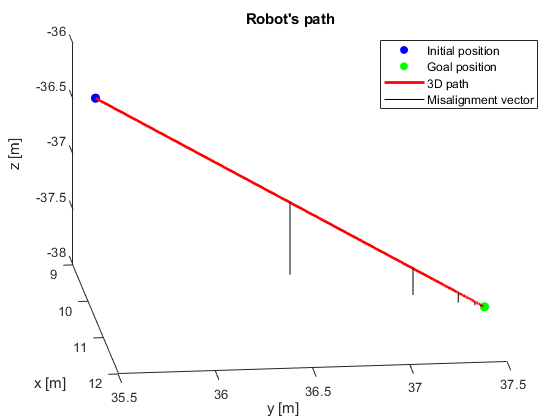
\includegraphics[width=0.7\linewidth]{images/Ex1/HorAtt_Disabled_SameStartpos_SameEndpos_Path}
	\caption{Here we can see that the robot reaches the goal position and that the misalignment vector shrinks towards zero.}
	\label{fig:q2case1c}
\end{figure}

{\large \textbf{Case 2}} \\
In this case the target configuration has roll and pitch angles both equal to $ \pi/3 $, so the Vehicle Position and Attitude task tries to rotate the robot in order to fulfill its objective, but, since the Horizontal Attitude task is enabled with higher priority, the robot can't reach the final configuration. In this case we have two conflicting tasks, but since the Horizontal Attitude one has higher priority the robot will try to stay as horizontal as possible: nevertheless, the robot will remain a bit tilted since this task is of inequality type (it becomes inactive when the norm of the misalignment vector is less than about half a degree).

\begin{figure}[H]
	\centering
	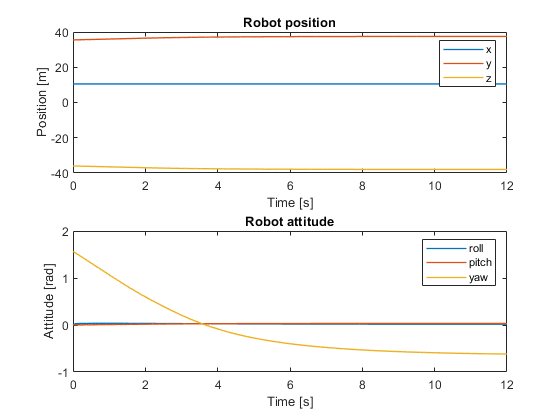
\includegraphics[width=0.7\linewidth]{images/Ex1/HorAtt_Enabled_SameStartpos_DifferentEndpos_PosAndAtt}
	\caption{The robot moves in the Y and Z directions, but the attitude doesn't converge to the desired one.}
	\label{fig:q2case2a}
\end{figure}
\begin{figure}[H]
	\centering
	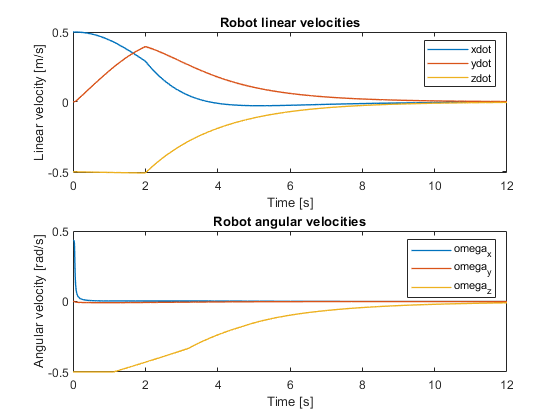
\includegraphics[width=0.7\linewidth]{images/Ex1/HorAtt_Enabled_SameStartpos_DifferentEndpos_LinAngVelocities}
	\caption{The robot velocities converge to zero after a while.}
	\label{fig:q2case2b}
\end{figure}
\begin{figure}[H]
	\centering
	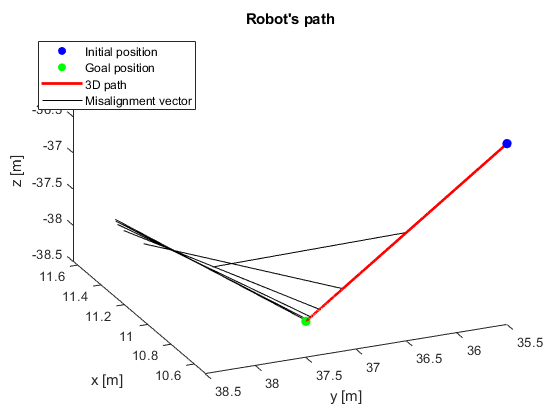
\includegraphics[width=0.7\linewidth]{images/Ex1/HorAtt_Enabled_SameStartpos_DifferentEndpos_Path}
	\caption{The robot can reach the goal position, but the misalignment vector keeps growing.}
	\label{fig:q2case2c}
\end{figure}
\begin{figure}[H]
	\centering
	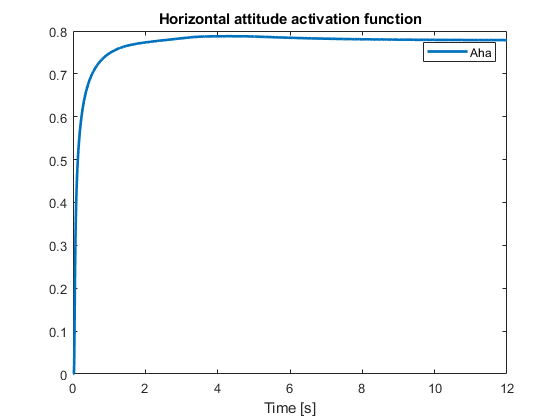
\includegraphics[width=0.7\linewidth]{images/Ex1/HorAtt_Enabled_SameStartpos_DifferentEndpos_ActivFunct}
	\caption{The activation function of the Horizontal Attitude task almost immediately reaches an high value, but it can't go back to zero since the robot has conflicting goals.}
	\label{fig:q2case2d}
\end{figure}

{\large \textbf{Case 3}} \\
Now both the initial configuration and the target one have pitch and roll angles equal to $ \pi/3 $: if the Horizontal Attitude wasn't enabled then the robot would only change its yaw angle and move linearly towards the goal, since the initial and the target pitch and roll angles are the same. In this case Horizontal Attitude is enabled, so this task tries to rotate the robot, whereas the Vehicle Position and Attitude one tries to keep the robot from rotating. The robot will reach the target position, but since the Horizontal Attitude task has higher priority, it will prevent the robot from reaching the target attitude.

\begin{figure}[H]
	\centering
	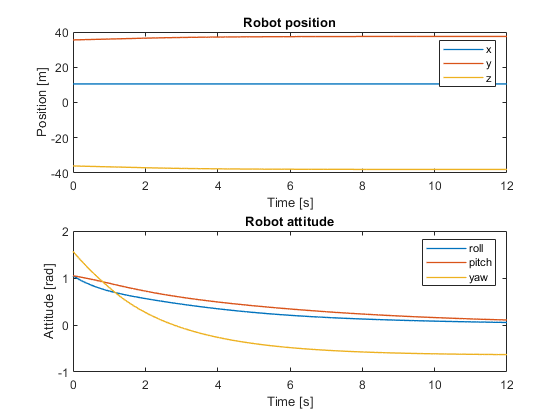
\includegraphics[width=0.7\linewidth]{images/Ex1/HorAtt_Enabled_DifferentStartpos_DifferentEndpos_PosAndAtt}
	\caption{We can see that the pitch and roll angles start from $ \pi/3 $ and converge near to 0: the robot moves in Y and Z, reaching the goal position.}
	\label{fig:q2case3a}
\end{figure}
\begin{figure}[H]
	\centering
	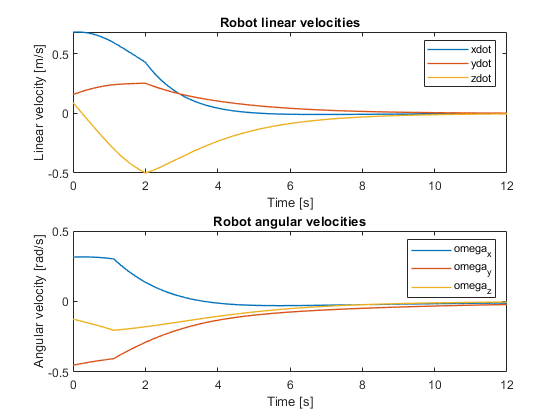
\includegraphics[width=0.7\linewidth]{images/Ex1/HorAtt_Enabled_DifferentStartpos_DifferentEndpos_LinAngVelocities}
	\caption{The robot rotates quite fast in the first 2-3 seconds, but then the angular velocities converge to zero. We can see a different $\dot{z}$ with respect to other cases since the robot is initially tilted.}
	\label{fig:q2case3b}
\end{figure}
\begin{figure}[H]
	\centering
	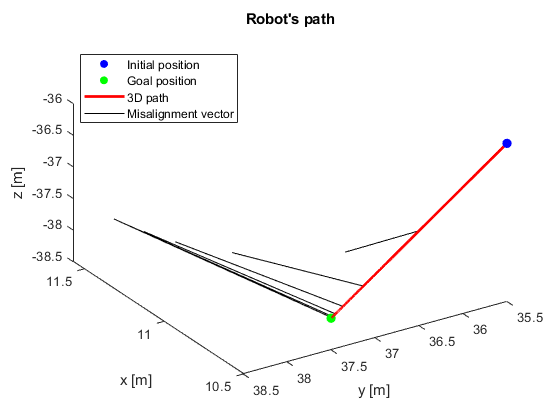
\includegraphics[width=0.7\linewidth]{images/Ex1/HorAtt_Enabled_DifferentStartpos_DifferentEndpos_Path}
	\caption{The robot reaches the goal position, but the misalignment vector continues to grow.}
	\label{fig:q2case3c}
\end{figure}
\begin{figure}[H]
	\centering
	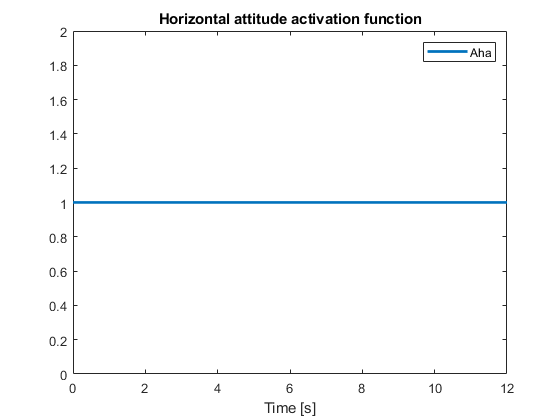
\includegraphics[width=0.7\linewidth]{images/Ex1/HorAtt_Enabled_DifferentStartpos_DifferentEndpos_ActivFunct}
	\caption{The activation function is always 1 since the norm of the misalignment vector is always bigger than the maximum allowed value.}
	\label{fig:q2case3d}
\end{figure}


\subsubsection{Q3: Swap the priorities between Horizontal Attitude and the Vehicle Position control task. Discuss the behaviour.}
Here I consider Case 2 and Case 3 which have been mentioned in the previous question, but with the Horizontal Attitude task at the bottom of the hierarchy.

{\large \textbf{Case 2}} \\
In the previous question, the robot had conflicting goals and the safety one was considered the most important: now we still have conflicting goals, but the most important one is that the robot should reach the target configuration. Since the Horizontal Attitude task won't have much effect on the robot, it will reach the target configuration without any problem.
\begin{figure}[H]
	\centering
	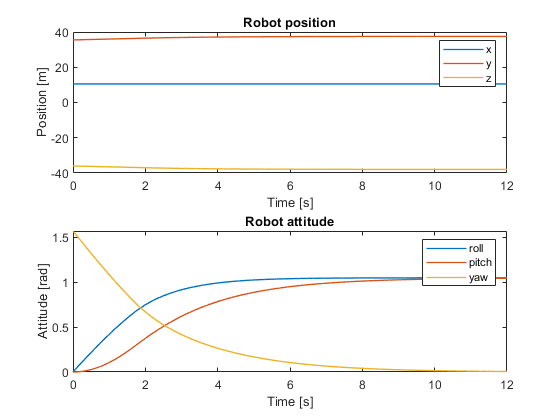
\includegraphics[width=0.7\linewidth]{images/Ex1/HorAtt_LowPrio_SameStartpos_DifferentEndpos_PosAndAtt}
	\caption{The robot configuration converges to the target one.}
	\label{fig:q3case2a}
\end{figure}
\begin{figure}[H]
	\centering
	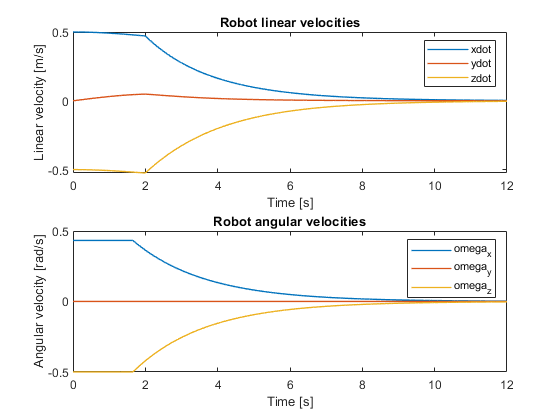
\includegraphics[width=0.7\linewidth]{images/Ex1/HorAtt_LowPrio_SameStartpos_DifferentEndpos_LinAngVelocities}
	\caption{The robot velocities converge to zero after a brief transient period.}
	\label{fig:q3case2b}
\end{figure}
\begin{figure}[H]
	\centering
	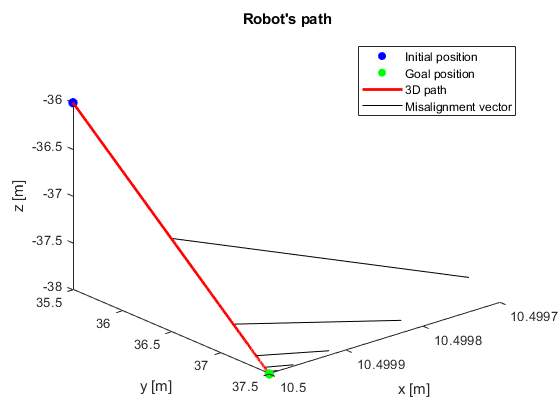
\includegraphics[width=0.7\linewidth]{images/Ex1/HorAtt_LowPrio_SameStartpos_DifferentEndpos_Path}
	\caption{The robot reaches the target position and the misalignment vector shrinks towards zero.}
	\label{fig:q3case2c}
\end{figure}
\begin{figure}[H]
	\centering
	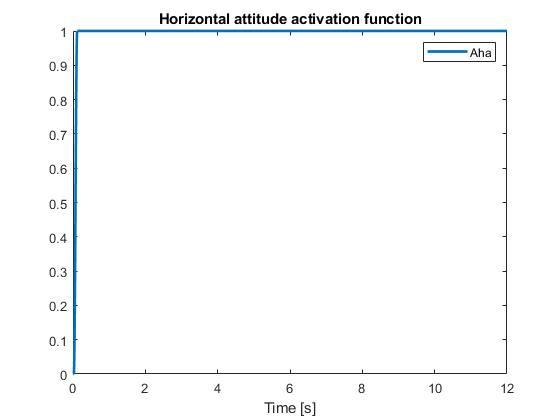
\includegraphics[width=0.7\linewidth]{images/Ex1/HorAtt_LowPrio_SameStartpos_DifferentEndpos_ActivFunct}
	\caption{The value of the activation value is almost always 1 since the task doesn't have effect on the robot.}
	\label{fig:q3case2d}
\end{figure}


{\large \textbf{Case 3}} \\
In the previous question, the Horizontal Attitude task prevented the robot to reach the target attitude: now this task won't have effect, allowing the robot to reach the target configuration.

\begin{figure}[H]
	\centering
	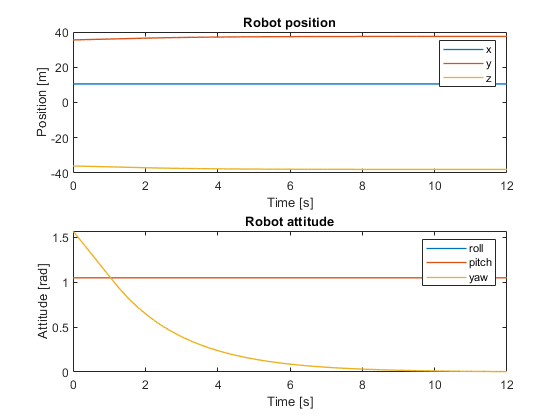
\includegraphics[width=0.7\linewidth]{images/Ex1/HorAtt_LowPrio_DifferentStartpos_DifferentEndpos_PosAndAtt}
	\caption{}
	\label{fig:q3case3a}
\end{figure}
\begin{figure}[H]
	\centering
	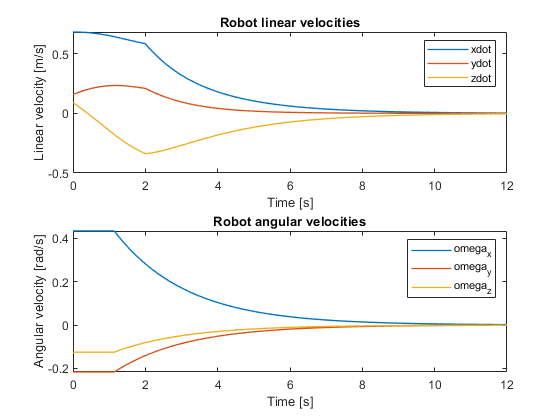
\includegraphics[width=0.7\linewidth]{images/Ex1/HorAtt_LowPrio_DifferentStartpos_DifferentEndpos_LinAngVelocities}
	\caption{}
	\label{fig:q3case3b}
\end{figure}
\begin{figure}[H]
	\centering
	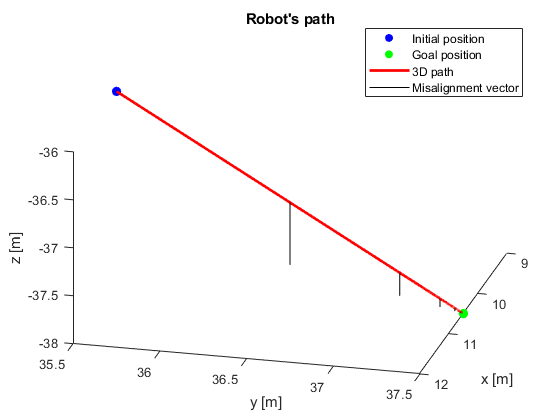
\includegraphics[width=0.7\linewidth]{images/Ex1/HorAtt_LowPrio_DifferentStartpos_DifferentEndpos_Path}
	\caption{}
	\label{fig:q3case3c}
\end{figure}
\begin{figure}[H]
	\centering
	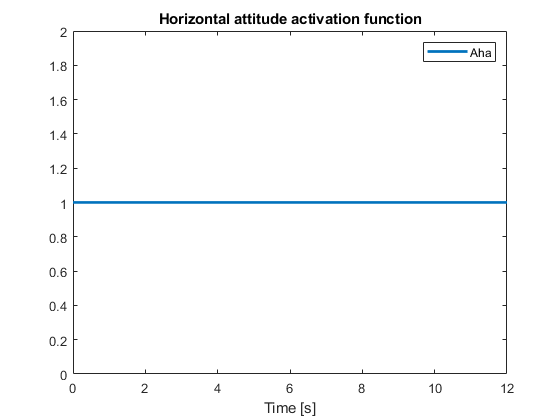
\includegraphics[width=0.7\linewidth]{images/Ex1/HorAtt_LowPrio_DifferentStartpos_DifferentEndpos_ActivFunct}
	\caption{}
	\label{fig:q3case3d}
\end{figure}


\subsubsection{Q4: What is the behaviour if the Tool Position control task is active and what if it is disabled? Which of the settings should be used for a Safe Waypoint Navigation action? Report the final hierarchy of tasks (and their priorities, see the template table in the introduction) which makes up the Safe Waypoint Navigation action.}


\subsection{Adding a safety minimum altitude control objective}
Initialize the vehicle at the position:
\begin{displaymath}
\begin{bmatrix} 48.5 & 11.5 & -33 & 0 & 0 &-\pi/2\end{bmatrix}^\top
\end{displaymath}
Choose as target point for the vehicle position the following one:
\begin{displaymath}
\begin{bmatrix} 50 & -12.5 & -33 & 0 & 0 & -\pi/2 \end{bmatrix}^\top
\end{displaymath}

Goal: Implement a task to control the altitude from the seafloor. Check that at all times the minimum distance from the seafloor is guaranteed.


\subsubsection{Q1: Report the new hierarchy of tasks of the Safe Waypoint Navigation and their priorities. Comment how you choose the priority level for the minimum altitude.}

\subsubsection{Q2: What is the Jacobian relationship for the Minimum Altitude control task? Report the formula for the desired task reference generation, and the activation thresholds.}

\subsubsection{Q3: Try imposing a minimum altitude of 1, 5, 10 m respectively. What is the behaviour? Does the vehicle reach its final goal in all cases?}

\subsubsection{Q4: How was the sensor distance processed to obtain the altitude measurement? Does it work in all cases or some underlying assumptions are implicitly made?}

\clearpage

\section{Exercise 2: Implement a Basic “Landing” Action.}
\subsection{Adding an altitude control objective}
Initialize the vehicle at the position:
\begin{displaymath}
\begin{bmatrix} 10.5 & 37.5 & -38 & 0 & -0.06 & 0.5 \end{bmatrix}^\top
\end{displaymath}

Goal: add a control task to regulate the altitude to zero.

\subsubsection{Q1: Report the hierarchy of task used and their priorities to implement the Landing Action. Comment how you choose the priority level for the altitude control task.}

\subsubsection{Q2: What is the Jacobian relationship for the Altitude control task? How was the task reference computed?}

\subsubsection{Q3: how does this task differs from a minimum altitude control task?}

\subsection{Adding mission phases and change of action}
Initialize the vehicle at the position:
\begin{displaymath}
\begin{bmatrix} 8.5 & 38.5 & -36 & 0 & -0.06 & 0.5 \end{bmatrix}^\top
\end{displaymath}
Use a "safe waypoint navigation action" to reach the following position:
\begin{displaymath}
\begin{bmatrix} 10.5 & 37.5 & -38 & 0 & -0.06 & 0.5 \end{bmatrix}^\top
\end{displaymath}
When the position has been reached, land on the seafloor using the basic "landing" action.

\subsubsection{Q1: Report the unified hierarchy of tasks used and their priorities.}

\subsubsection{Q2: How did you implement the transition from one action to the other?}

\clearpage

\section{Exercise 3: Improve the “Landing” Action}
\subsection{Adding an alignment to target control objective}
If we use the landing action, there is no guarantee that we land in from of the nodule/rock. We need to add additional constraints to make the vehicle face the nodule. The position of the rock is contained in the variable \texttt{rock\_center}.

Initialize the vehicle at the position:
\begin{displaymath}
\begin{bmatrix} 8.5 & 38.5 & -36 & 0 & -0.06 & 0.5 \end{bmatrix}^\top
\end{displaymath}
Use a "safe waypoint navigation action" to reach the following position:
\begin{displaymath}
\begin{bmatrix} 10.5 & 37.5 & -38 & 0 & -0.06 & 0.5 \end{bmatrix}^\top
\end{displaymath}
Then land, aligning to the nodule.

Goal: Add an alignment task between the longitudinal axis of the vehicle ($x$ axis) and the nodule target. In particular, the $x$ axis of the vehicle should align to the projection, on the inertial horizontal plane, of the unit vector joining the vehicle frame to the nodule frame.

\subsubsection{Q1: Report the hierarchy of tasks used and their priorities in each action. Comment the behaviour.}

\begin{table}[htb]
	\caption{Task hierarchy for the set of actions used to move the vehicle near the target and then align it.}
	\begin{itemize}
		\item Action 1 ($\mathcal{A}_{1}$) : Safe Navigation
		\item Action 2 ($\mathcal{A}_{2}$) : Aligned Landing
	\end{itemize}
	\label{tb_align:actions_table}
	% Horizontal attitude = 2
	% Vehicle position = 3
	% Vehicle attitude = 4
	% Vehicle minimum altitude = 5
	% Vehicle altitude control = 6
	% Horizontal alignment to target = 7
	% A1:[2, 6, 7]
	% A2:[2, 3, 4, 5]
	\begin{center}
		\footnotesize
		\begin{tabular}{cccc}
			\toprule
			Task & Type & $\mathcal{A}_{1}$ & $\mathcal{A}_{2}$ \\
			\midrule
			Horizontal Attitude             & I & 2 & 1 \\
			\hdashline
			Vehicle Position				& E & 3 &   \\
			\hdashline
			Vehicle Attitude                & E & 4 &   \\
			\hdashline
			Vehicle Minimum Altitude        & I & 1 &   \\
			\hdashline
			Vehicle Altitude Control        & E &   & 3 \\
			\hdashline
			Alignment to Target             & E &   & 2 \\
			
			\bottomrule
		\end{tabular}
	\end{center}
\end{table}% %

The vehicle initially starts from a point quite high with respect to the ground and some meters away from the target ({\small\(\begin{bmatrix} 8.5 & 38.5 & -36 & 0 & -0.06 & 0.5 \end{bmatrix}^\top\)})\\
The first action performed is the Safe Navigation, which leads the vehicle to move to a specified point using two safety tasks, which have the top priority, the Minimum Altitude Task and the Horizontal Attitude Task, and two tasks to move the vehicle to the goal, the Vehicle Position and Vehicle Attitude Tasks.\\
When the linear distance between the vehicle and the goal position ({\small \(\begin{bmatrix} 10.5 & 37.5 & -38 & 0 & -0.06 & 0.5 \end{bmatrix}^\top\) }) falls under $0.1 m$, the action changes and the vehicle begins the landing. This second action is called Aligned Landing and it is composed by three tasks, one safety task which is the Horizontal Attitude, and the two tasks for landing in front of the rock: Vehicle Minimum Altitude that makes the vehicle land on the sea floor, and the Alignment to Target, which makes the vehicle $x$ axis align to the projection on the inertial horizontal plane of the unit vector joining the vehicle frame to the nodule frame.\\ 
The vehicle successfully manages to land right in front of the rock and with the expected alignment, as shown in Figure \ref{im:v_align_land}.

\begin{figure}[H]
	\centering
	{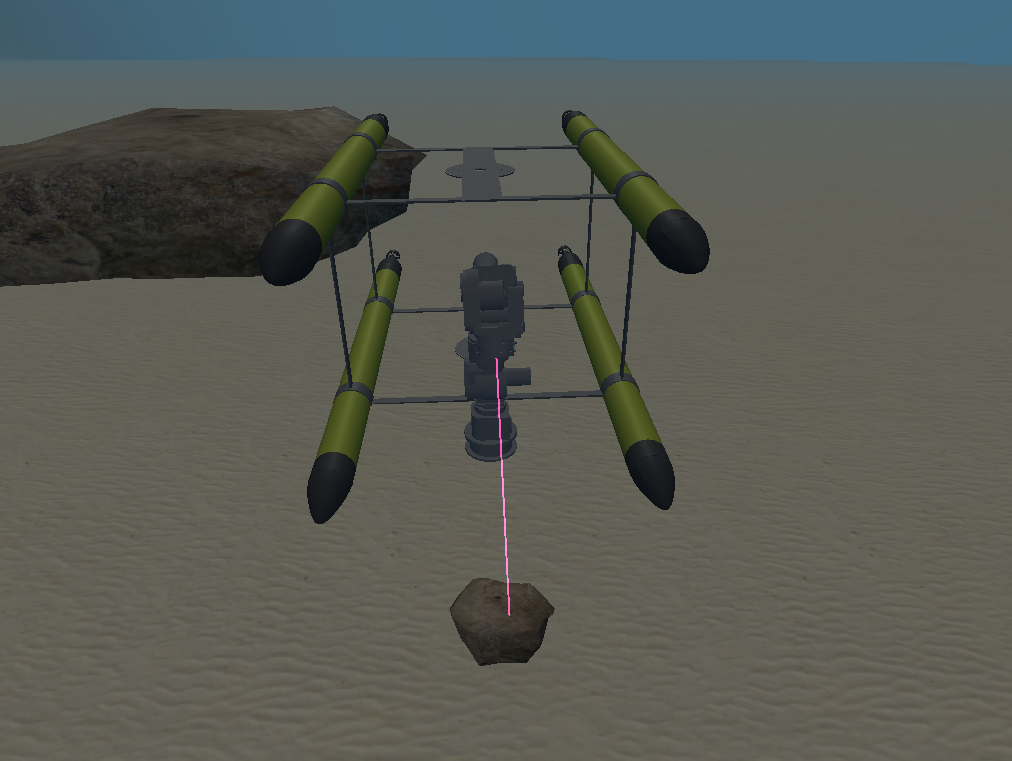
\includegraphics[scale=0.35]{vehicle_aligned_landing.png}}
	\caption{Simulation showing the vehicle after landing in front of the rock.}
	\label{im:v_align_land}
\end{figure}

Here the path that the robot performs is shown in a 3D plot, joint with the misalignment vector between the x axis of the robot and the projection on the inertial horizontal plane of the unit vector joining the vehicle frame to the rock frame.

\begin{figure}[H]
	\centering
	{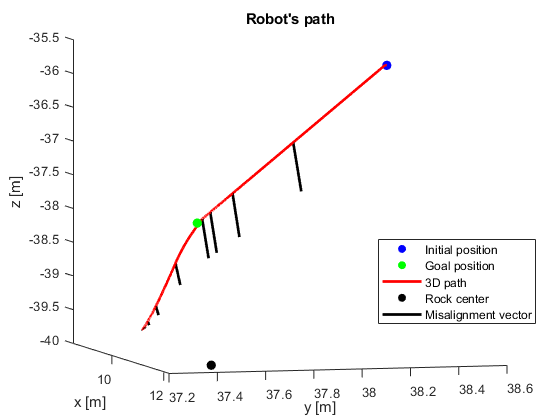
\includegraphics[scale=0.65]{plot_3_1_misalignment.png}}
	\caption{Plot of the Vehicle path.}
	\label{im:v_path_align_land}
\end{figure}

\subsubsection{Q2: What is the Jacobian relationship for the Alignment to Target control task? How was the task reference computed?}
The first thing to do is to calculate the vector to which the vehicle axis have to align, that is the distance between the vehicle frame origin  and the target (in the world frame), projected on the horizontal plane of the inertial frame. 
$$ ^wd = ^wP - ^wO_v$$
$$^wd_{proj} = ^wd - ((^wd^T \cdot ^wk_w) \cdot ^wk_w)$$

Then the misalignment vector (\(\rho\)) between the x-axis of the vehicle and the \(d_{proj}\) versor (\(n_{d_{proj}}=\frac{d_{proj}}{\|d_{proj}\|}\)) is calculated using the Reduced Versor Lemma, after having projected both versors on the vehicle frame.
$$^v\rho = \theta n$$

The Jacobian relationship obtained is the following:

$$ \begin{bmatrix} \bm{\omega_x}   \\ \bm{\omega_y} \\ \bm{\omega_z} \end{bmatrix} = J_{ha} \bm{\dot{y}}$$
$$ \begin{bmatrix} \bm{\omega_x}   \\ \bm{\omega_y} \\ \bm{\omega_z} \end{bmatrix} = n \cdot \begin{bmatrix} \bm{0}_{[3x7]} & -\frac{1}{\|^vd_{proj}\|^2}[^vd_{proj}\wedge] & -\bm{I}_{[3x3]} \end{bmatrix} \begin{bmatrix} \bm{q}   \\ \bm{\textit{v}} \\ \bm{\omega} \end{bmatrix} $$

The task reference is computed using the norm of the misalignment vector, $\theta$. The desired value in this case is \(0\), because we want the two vectors to be aligned.

\begin{lstlisting}
	uvms.xdot.horAlign = Saturate(0.5 * (0 - uvms.theta), 0.5);
\end{lstlisting}

\subsubsection{Q3: Try changing the gain of the alignment task. Try at least three different values, where one is very small. What is the observed behaviour? Could you devise a solution that is gain-independent guaranteeing that the landing is accomplished aligned to the target?}
The initial alignment task gain is saturated at 0.5, then we tried to change its value with three different ones: 0.05, 0.2, 0.4 ,0.7.

\begin{figure}[H]
	\centering
	\subfigure[Position of the vehicle when it approches the ground with gain = \(0.05\)]
	{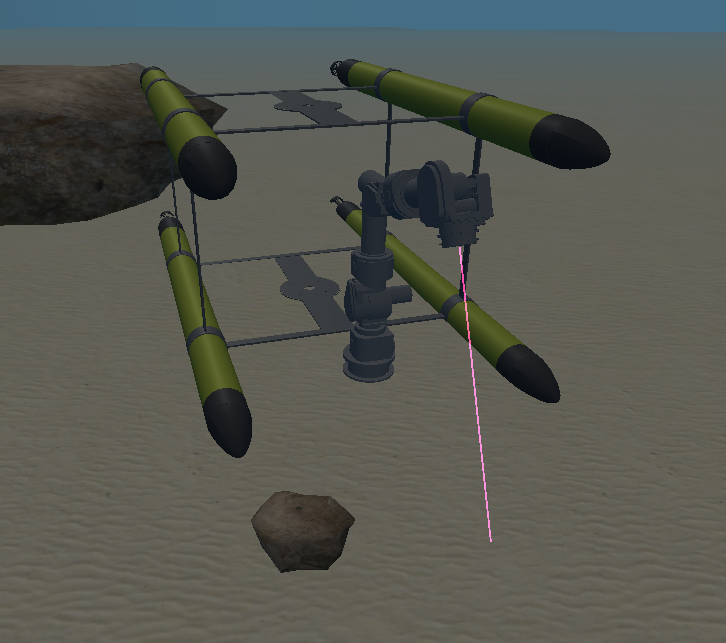
\includegraphics[width=60mm]{3_1_3_gain0_05_landed.png}}
	\hspace{10mm}
	\subfigure[Path of the vehicle and misalignment vector with gain = \(0.05\)]
	{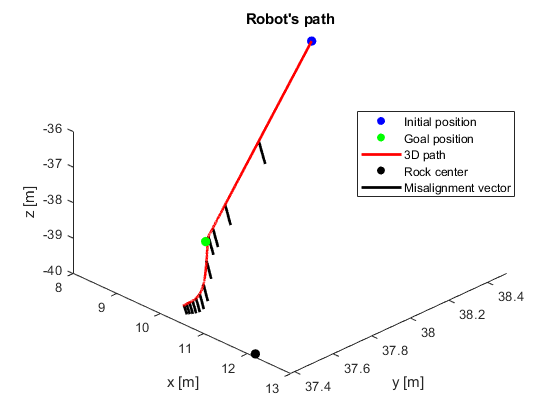
\includegraphics[width=70mm]{3_1_3_gain0_05.png}}
	\label{im:v_land_gain0_05}
\end{figure} 

\begin{figure}[H]
	\centering
	\subfigure[Position of the vehicle when it approches the ground with gain = \(0.2\)]
	{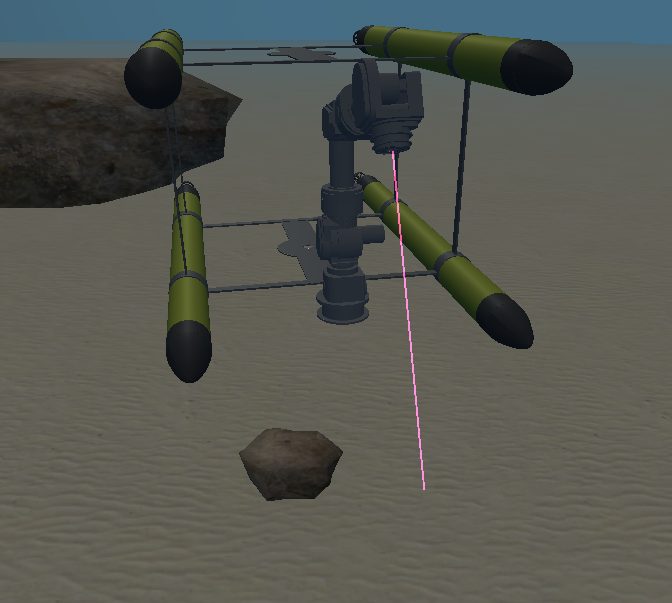
\includegraphics[width=60mm]{3_1_3_gain0_2_landed.png}}
	\hspace{10mm}
	\subfigure[Path of the vehicle and misalignment vector with gain = \(0.2\)]
	{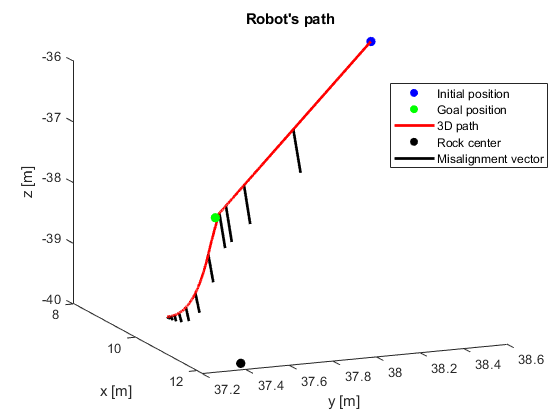
\includegraphics[width=70mm]{3_1_3_gain0_2.png}}
	\label{im:v_land_gain0_2}
\end{figure} 

\begin{figure}[H]
	\centering
	\subfigure[Position of the vehicle when it approches the ground with gain = \(0.4\)]
	{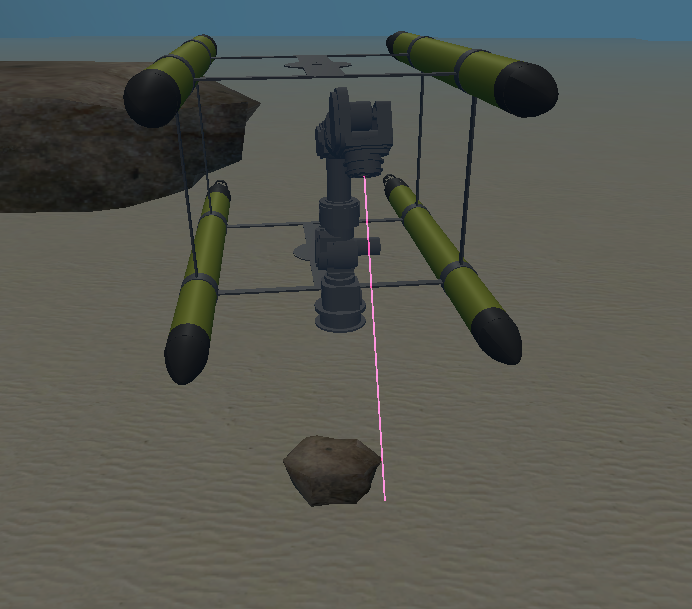
\includegraphics[width=60mm]{3_1_3_gain0_4_landed.png}}
	\hspace{10mm}
	\subfigure[Path of the vehicle and misalignment vector with gain = \(0.4\)]
	{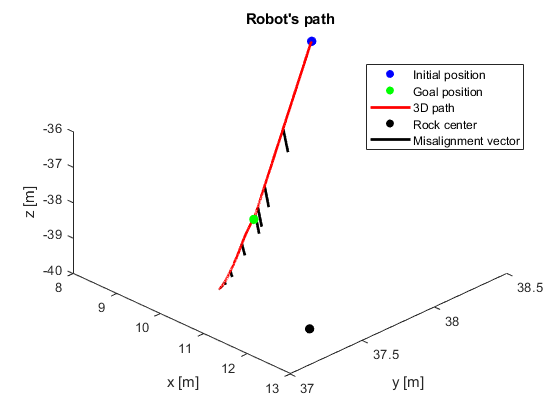
\includegraphics[width=70mm]{3_1_3_gain0_4.png}}
	\label{im:v_land_gain0_4}
\end{figure} 

\begin{figure}[H]
	\centering
	\subfigure[Position of the vehicle when it approches the ground with gain = \(0.7\)]
	{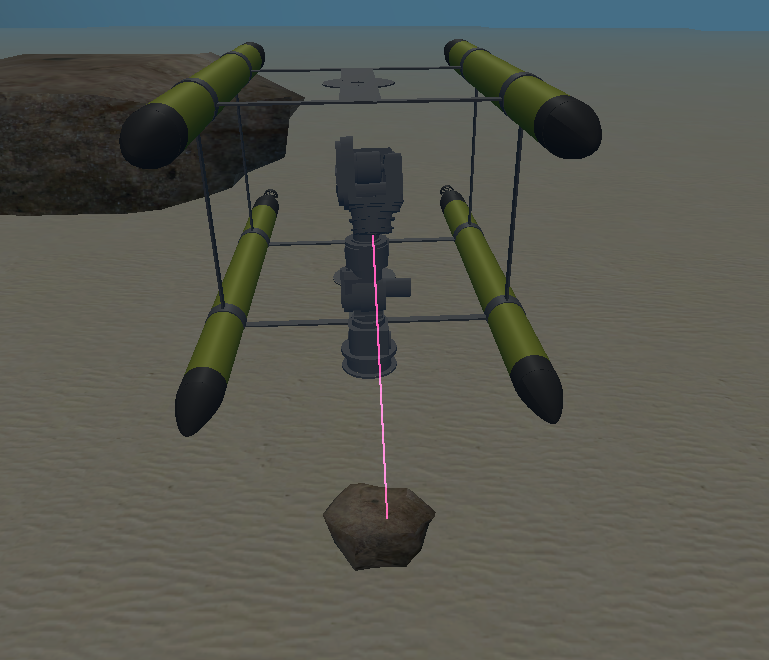
\includegraphics[width=60mm]{3_1_3_gain0_7_landed.png}}
	\hspace{10mm}
	\subfigure[Path of the vehicle and misalignment vector with gain = \(0.7\)]
	{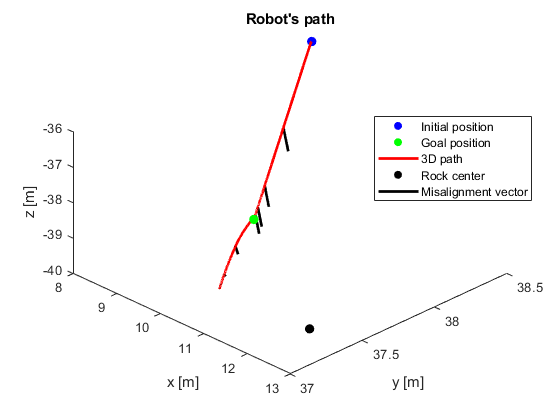
\includegraphics[width=70mm]{3_1_3_gain0_7.png}}
	\label{im:v_land_gain0_7}
\end{figure} 

The behaviour of the vehicle changes when the gain value is modified: the smaller the gain, the harder it is for the vehicle to reach the correct alignment with \(d_{proj}\). As it can be seen in the images above, while the time used by the robot to reach the sea floor remains the same, increasing the gain makes it reach different configurations when approaching the sea floor.\\
For gain values smaller than about \(0.2\), the misalignment vector fails to become a null vector, as you can clearly see in images (b) and (d), so the vehicle is not able to align to the target in time. In the other two cases instead the vehicle manages to align in time to the target, even if, for gain = \(0.4\).
This shows that this solution is heavily gain-dependent, so we need to think about a solution to ensure that the alignment is always achieved.
What we thought was to add a new Action in between the two actual ones that is activated when the vehicle reaches the goal position for the Safe Navigation action. This new Action is composed by two tasks, horizontal attitude for safety and the horizontal aligning to the target. This action is performed until the module of the misalignment vector, $\theta$, becomes lower than \(0.02 \) \({rad}\).\\
Then, the vehicle start the landing, but the misalignment vector between its x-axis and \(n_{d_{proj}}\) is already very close to zero, so it is guaranteed that it will land aligned to the target, independently from the gain of the alignment task.
\begin{figure}[H]
	\centering
	\subfigure[Robot path and misalignment vector with gain = \(0.1\) (gain independent)]
	{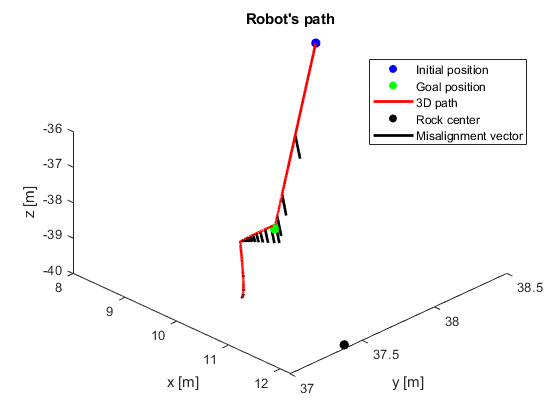
\includegraphics[width=80mm]{3_1_3_gain0_1_independent.png}}
	\label{im:v_land_gain0_1_ind}
\end{figure} 
The behaviour obtained shows that the vehicle manages to land aligned with the target even if the gain value is very low.
 
\subsubsection{Q4: After the landing is accomplished, what happens if you try to move the end-effector? Is the distance to the nodule sufficient to reach it with the end-effector? Comment the observed behaviour. If, after landing, the nodule is not in the manipulator's workspace, how would you solve this problem to guarantee it?}

In order to move the end effector after landing is accomplished, we need to introduce a new action, that we called Grasp Object, that will be performed after the altitude previous action is concluded, that is when the vehicle altitude from the sea floor is lower than \(0.1 m\). This action is composed by three tasks: 
\begin{itemize}
	\item the Horizontal Attitude, for safety
	\item the Vehicle Altitude Control, that is the same task present in the landing action, which is needed to let the vehicle remain at the same altitude from the sea floor
	\item the Tool Position Control, that is needed to move the end effector of the arm on the desired position
\end{itemize}
After the landing is accomplished, the robot arm starts moving towards the target and, since there is no constraint task on the vehicle velocities, the body shifts laterally and leans froward, following the arm movement, until the end effector reaches the goal position.

\begin{figure}[H]
	\centering
	\subfigure[Position of the vehicle after the grasping is completed]
	{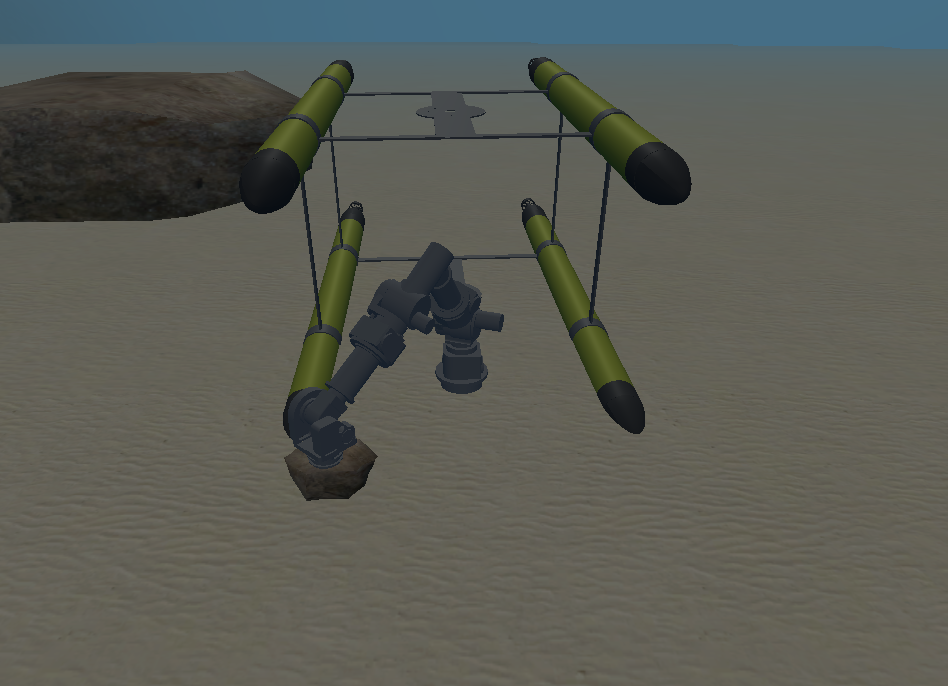
\includegraphics[width=70mm]{3_1_4_vehic_grasp_sim.png}}
	\hspace{10mm}
	\subfigure[Path of the vehicle and misalignment vector ]
	{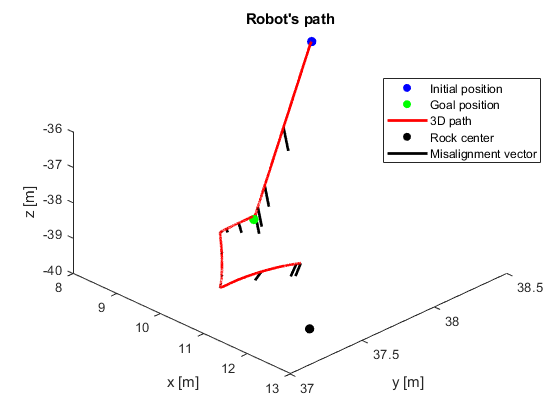
\includegraphics[width=70mm]{3_1_4_vehic_grasp.png}}
	\label{im:v_land_grasp}
\end{figure} 
So I observed that in this case the distance to the nodule is sufficient to reach it with the end-effector. Nevertheless it is not guaranteed to happen, so it is a good idea to add a new task that ensures that the target will be in the manipulator space when the landing is accomplished.

\clearpage

\section{Exercise 4: Implementing a Fixed-base Manipulation Action}
\subsection{Adding non-reactive tasks}
To manipulate as a fixed based manipulator, we need to constraint the vehicle to not move, otherwise the tool frame position task will make the vehicle move.

Goal: Add a constraint task that fixes the vehicle velocity to zero. Land on the seafloor. Try reaching the rock position with the end-effector, and observe that the vehicle does not move.

\subsubsection{Q1: Report the hierarchy of tasks used and their priorities in each action. At which priority level did you add the constraint task?}

\subsubsection{Q2: What is the Jacobian relationship for the Vehicle Null Velocity task? How was the task reference computed?}

\subsubsection{Q3: Suppose that the vehicle is floating, i.e. not landed on the seafloor. What would happen, if due to currents, the vehicle moves?}


\subsection{Adding a joint limit task}
Let us now constrain the arm with the actual joint limits. The vector variables \texttt{uvms.jlmin} and \texttt{uvms.jlmax} contain the maximum and minimum values respectively.

Goal: Add a joint limits avoidance task. Land on the seafloor. Try reaching the rock position with the end-effector, and observe that the vehicle does not move and that all the joints are within their limits.

\subsubsection{Q1: Report the hierarchy of tasks used and their priorities in each action. At which priority level did you add the joint limits task?}

\subsubsection{Q2: What is the Jacobian relationship for the Joint Limits task? How was the task reference computed?}

\clearpage
\section{Exercise 5: Floating Manipulation}
\subsection{Adding an optimization control objective}
Use the DexROV simulation for this exercise.

The goal is to try to optimize the joint positions, if possible, to keep the first four joints in a "preferred shape", represented by the following vector
\begin{displaymath}
\begin{bmatrix}-0.0031 & 1.2586 & 0.0128 & -1.2460 \end{bmatrix}^\top
\end{displaymath}

Goal: Add an optimization objective to keep the first four joints of the manipulator in the preferred shape. Observe the behaviour with and without the task

\subsubsection{Q1: Report the hierarchy of tasks used and their priorities in each action. At which priority level did you add the optimization task?}

\subsubsection{Q2: What is the Jacobian relationship for the Joint Preferred Shape task? How was the task reference computed?}

\subsubsection{Q3: What is the difference between having or not having this objective?}

\subsection{Adding mission phases}
Let us now structure the mission in more than one phase. In the first phase, exploit the previous exercises, and implement a safe waypoint navigation. Move the vehicle to a location close to the current defined end-effector goal position, just slightly above it. Then, trigger a change of action and perform floating manipulation.

Goal: introduce mission phases in the floating manipulation scenario. Observe the difference.

\subsubsection{Q1: Report the unified hierarchy of tasks used and their priorities. Which task is active in which phase/action?}

\subsubsection{Q2: What is the difference with the previous simulation (still in exercise 5), where only one action was used?}

\clearpage
\section{Exercise 6: Floating Manipulation with Arm-Vehicle Coordination Scheme}
\subsection{Adding the parallel arm-vehicle coordination scheme}
Let us now see how the two different subsystems (arm and vehicle) can be properly coordinate. Introduce in the simulation a sinusoidal velocity disturbance acting on the vehicle, and assume the actual vehicle velocity measurable. To do so, add a constant (in the inertial frame) velocity vector to the reference vehicle velocity before integrating it in the simulator.

Goal: modify the control part to implement the parallel arm-vehicle coordination scheme. Observe that, even with a disturbance acting on the vehicle, the end-effector can stay in the required constant position.

\subsubsection{Q1: Which tasks did you introduce to implement the parallel coordination scheme?}
In order to obtain the desired behavior we have introduced two kinds of disturbances, one linear and the other as angular velocity disturbance, expressed in the inertial frame. The vehicle suffers from these velocities, as they are added before integration. 
\begin{lstlisting}
%	Adding the disturbances
disturb = [0 0.025 0]';
disturb_ang = [0 0 0]';
disturb_ang = disturb_ang*0.5*sin(0.5*t*2*pi);
uvms.p_dot(1:3) = uvms.wTv(1:3,1:3)*disturb;
uvms.p_dot(4:6) = uvms.wTv(1:3,1:3)*disturb_ang;
    
% beware: p_dot should be projected on <v>
uvms.p = integrate_vehicle(uvms.p, uvms.p_dot, deltat);
\end{lstlisting}
This task objective is to keep the end effector position stable while the vehicle moves. As a result, the arm and the vehicle result as two different systems; specifically, the first could cope with incugruences in the second, but only in a limited way.
In order to cope with this disturbances we defined a new task called: armVehiCoord.
This task is placed with the highest hierarchy, limiting the manifold of solution to the ones accounting for the vehicle velocities. In fact, in order to decouple the two systems, we need to feed the arm with the vehicle velocities, the jacobian matrix accounts only for the vehicle velocities, disregarding the arm velocities.
$ \bm{\dot{x}} = \bm{J\dot{y}} $ which in this case becames 
$$ \bm{\dot{x}} = \begin{bmatrix} \bm{0}_{[6x7]} \\ \bm{I}_{[6x6]} \end{bmatrix} \begin{bmatrix} \bm{q}   \\ \bm{\textit{v}} \\ \bm{\omega} \end{bmatrix} $$

The task takes as a reference the velocities of the vehicle, as this is the input the arm has to compensate. Concerning the activation funtion, this is defined as an identity matrix, as the task is an equality one. 



\subsubsection{Q2: Show the plot of the position of the end-effector, showing that it is constant. Show also a plot of the velocities of the vehicle and of the arm.}
In the following images, the end effector position is plotted, showing the three cartesian components. The scale of the plots clearly states that the end effector position could be assumed as constant, as it only suffers from oscillation smaller than a millimiter. 

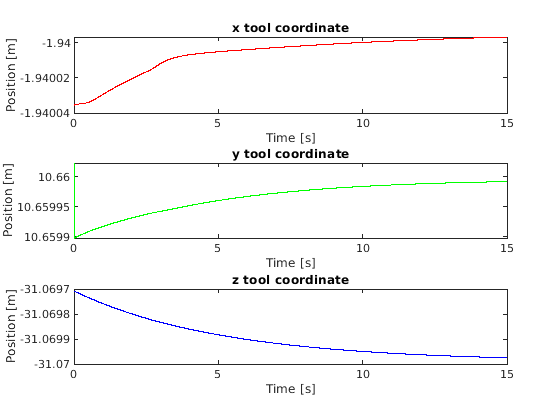
\includegraphics[width=\textwidth]{tool_coord}
\centering

The following image compares the vehicle velocities, expressed in the vehicle frame, and the velocites of the arm joints. The vehicle linear velocities show the effect of the linear disturbance, which brings a change in the vehicle velocities on x and y. 
The arm velocities are the resultant for the control of the end effector in its original position. 

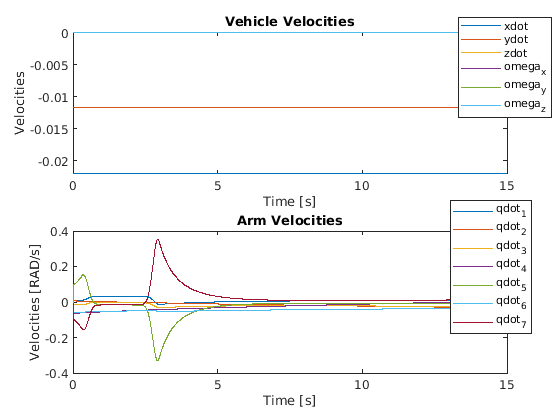
\includegraphics[width=\textwidth]{Vehicle_arm_volocities}
\centering



In this last image, we would like to show the evolution of the end effector velocities expressed in the inertial frame. The velocities start with a nonzero infinitesimal value, but they converge to zero in few seconds.

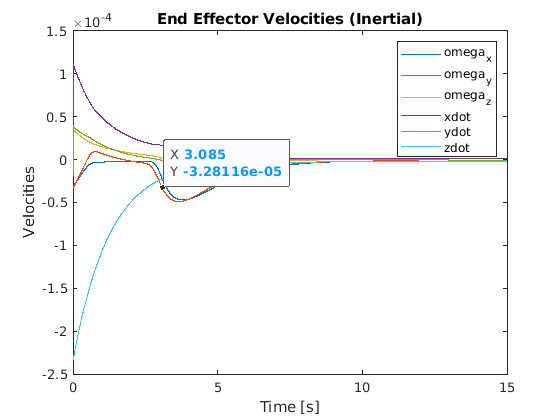
\includegraphics[width=\textwidth]{EE_velocities}
\centering


\subsubsection{Q3: What happens if the sinusoidal disturbance becomes too big? Try increasing the saturation value of the end-effector task if it is too low.}
If we add a sinusoidal disturbance, it deteriorates the ability of keeping the end effector still. The disturbance is added as described below. 
\begin{lstlisting}
%	Adding the disturbances
disturb = [0 0.0 0]';
disturb_ang = [0 1 0]';
disturb_ang = disturb_ang*0.2*sin(0.5*t*2*pi);
uvms.p_dot(1:3) = uvms.wTv(1:3,1:3)*disturb;
uvms.p_dot(4:6) = uvms.wTv(1:3,1:3)*disturb_ang;
\end{lstlisting}
However, as it can be seen in the following images, the end effector does not moves much. 
The following figure shows that the oscillations of the tool position are of the order of one millimiter, which can be considered as a acceptable result. 

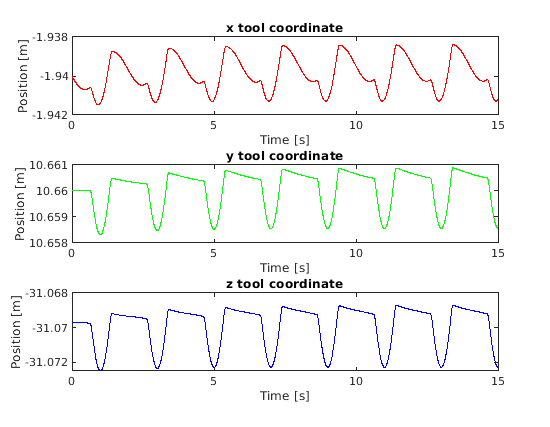
\includegraphics[width=\textwidth]{tool_coord_sinus_debole}
\centering

The following images compares the vehicle velocities with the joint rotational speed. 
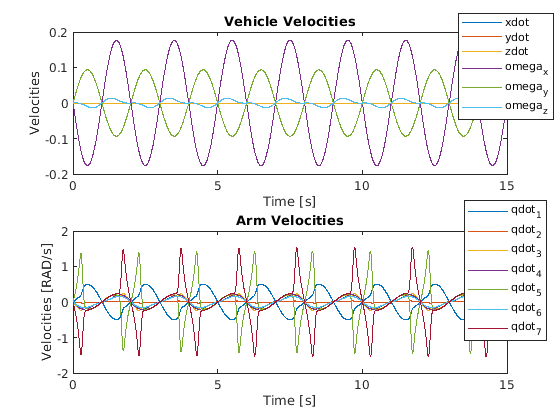
\includegraphics[width=\textwidth]{Vehicle_arm_volocities_sinus_debole}
\centering

Finally, this last image shows that the end effector velocities remains reasonable small. 
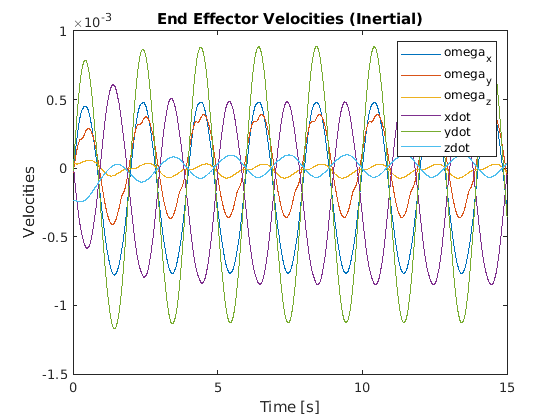
\includegraphics[width=\textwidth]{EE_velocities_sinus_debole}
\centering
 
However, if we increase the disturbance too much, the arms cannot cope with the disturbance in the vehicle. As a result, the displacement of the end effer are not negletable. Even if we increase the gain and the saturation of the tool control task, this is not sufficient to cancel the disturbannce.  The disturbance is added as described below.
\begin{lstlisting}
%	Adding the disturbances
    disturb = [0 0.0 0]';
    disturb_ang = [0 1 0]';
    disturb_ang = disturb_ang*1*sin(0.5*t*2*pi);
    uvms.p_dot(1:3) = uvms.wTv(1:3,1:3)*disturb;
    uvms.p_dot(4:6) = uvms.wTv(1:3,1:3)*disturb_ang;
\end{lstlisting}
The results of such a disturbance as shown in the images below.
First from this first image we can see that the end effecor is clearly moving from the 
desired position. The displacemnts on x reach almost 10 cm. 
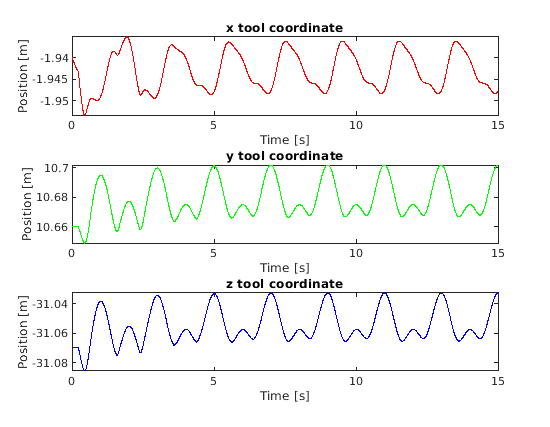
\includegraphics[width=\textwidth]{tool_coord_sinus_forte}
\centering

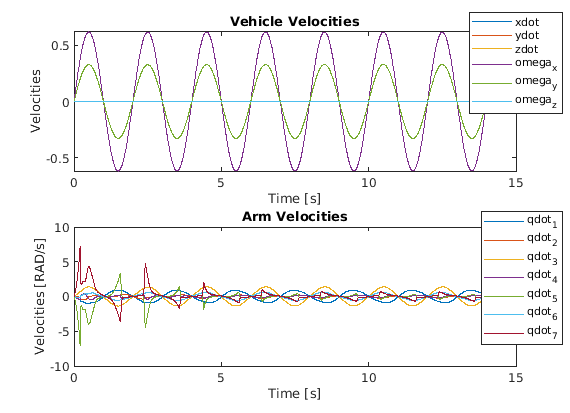
\includegraphics[width=\textwidth]{Vehicle_arm_volocities_sinus_forte}
\centering
Comparing the vehicle velocities with either the arm joints or end effector velocities, it is clear that in this case the task fails in its purpose. 
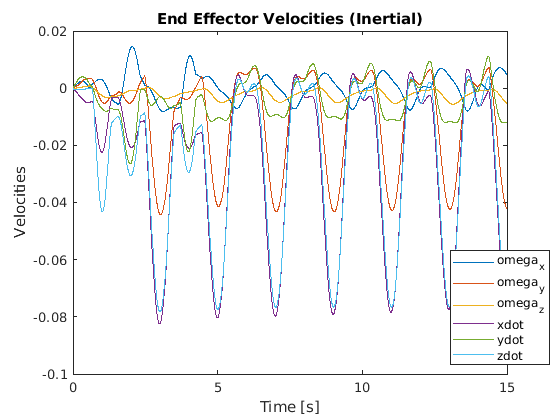
\includegraphics[width=\textwidth]{EE_velocities_sinus_forte}
\centering
















%\begin{figure}[t]
%	\centering
%	\subfloat[]{\includegraphics[height=7cm]{trident.jpg}}\label{fig:trident}
%	\subfloat[]{\includegraphics[height=7cm]{maris.jpg}}\label{fig:maris}
%	\caption{(a) TRIDENT UVMS (b) MARIS UVMS.}\label{fig:uvms_examples}
%\end{figure}



%		\begin{figure}[b]
%			\centering
%			\subfloat[]{\frame{\includegraphics[keepaspectratio,height=3cm]{trident1.eps}}}
%			\subfloat[]{\frame{\includegraphics[keepaspectratio,height=3cm]{trident2.eps}}}
%			\subfloat[]{\frame{\includegraphics[keepaspectratio,height=3cm]{trident3.eps}}}
%			\subfloat[]{\frame{\includegraphics[keepaspectratio,height=3cm]{trident4.eps}}}
%			\caption{Sequence of snapshots taken from the onboard camera during the TRIDENT final experiments.}
%			\label{fig_tri_trial_maiorca_img}
%		\end{figure}


\end{document}
